\documentclass[a0paper, portrait]{tikzposter}

\title{Distributional Gastronomics}
\author{Jonathan Oberl\"ander and Laura Bostan\\@L3viathan2142\quad\quad\quad @sarnthil}
\institute{Trento University}

\usepackage{booktabs}
\usepackage{amsmath}
\usepackage{array}

\usetheme{Simple}
\tikzposterlatexaffectionproofoff % no annoying logo

\begin{document}
    \maketitle
    \begin{columns}
        \column{0.5}
        \block{Distributional Gastronomics}{
            %Co-occurrence of ingredients with eachother in recipes
            \textbf{The distributional gastronomical hypothesis:} Similar ingredients will occur in similar contexts.
            \vspace{1cm}

            We present a distributional semantic model for recipes by building a representation of food ingredients and recipes in terms of co-occurrence vectors, recording their distributional pattern in a recipe corpus. We build a space for ingredients and two spaces for recipes.
        }
        \block{Obtaining a Vector Space from Recipes}{
            We utilize the recipe database crawled by \textbf{Open Recipes}. The list of ingredients per recipe plus its name was obtained, everything else discarded.

            We then unify ingredient names (cleaning artifacts and getting rid of units and amounts), to reduce the number of types from over 400,000 to just 6514.

        \vspace{2cm}

        \begin{center}
        \begin{tabular}{lr}
            \toprule
            \textbf{Number of recipes} & 172893\\
            \textbf{Number of ingredients (tokens in corpus)} & 1689892\\
            \textbf{Number of ingredients (types in corpus)} & 412858\\
            \textbf{Number of ingredients (types after unifying)} & 6514\\
            \bottomrule
        \end{tabular}
        \end{center}

        \vspace{2cm}

            In every recipe, we count each pair of ingredients as co-occurring, and build a large 6514-dimensional matrix.

        \vspace{2cm}

        \begin{center}
            \begin{tabular}{clcccc}
            \toprule
            & & 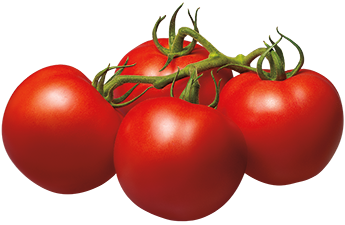
\includegraphics[height=1.5cm]{tomatoes.png}& 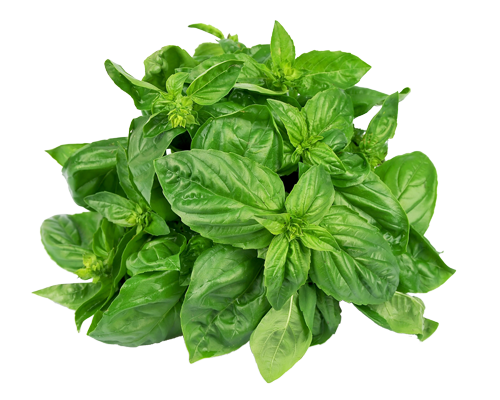
\includegraphics[height=1.5cm]{basil.png}& 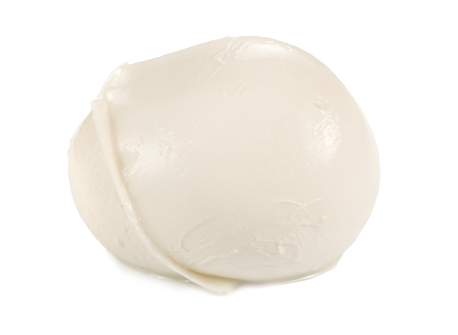
\includegraphics[height=1.5cm]{mozzarella.png} & 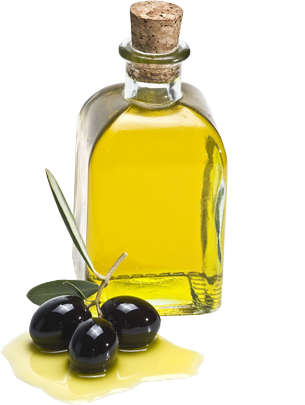
\includegraphics[height=1.5cm]{oliveoil.png} \\
            & & tomates & basil & mozzarella & olive oil\\
            \midrule
            \raisebox{-.3\height}{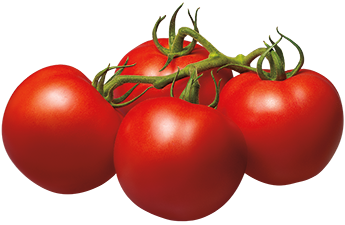
\includegraphics[height=1.5cm]{tomatoes.png}} &tomatoes & 1562 & 21 & 6 & 711\\
            \raisebox{-.3\height}{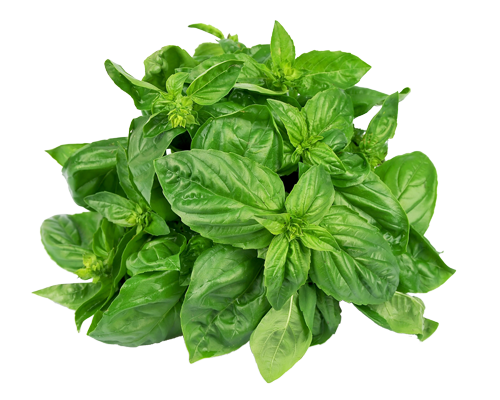
\includegraphics[height=1.5cm]{basil.png}} &basil & 21 & 434 & 13 & 239\\
            \raisebox{-.3\height}{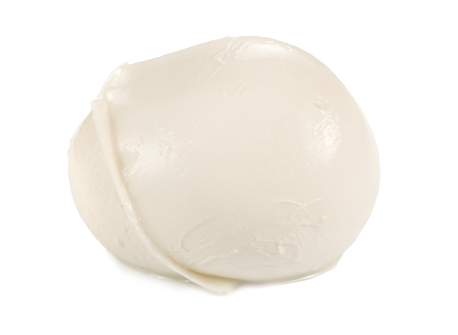
\includegraphics[height=1.5cm]{mozzarella.png}} &mozzarella & 6 & 13 & 149 & 95\\
            \raisebox{-.3\height}{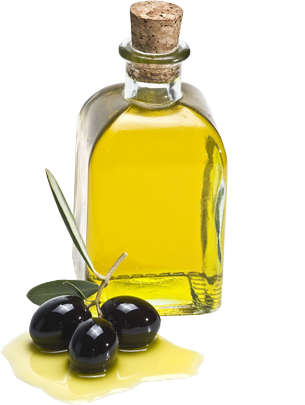
\includegraphics[height=1.5cm]{oliveoil.png}} &olive oil & 711 & 239 & 95 & 27659\\
            \bottomrule
        \end{tabular}
        \end{center}

        \vspace{2cm}

        After reweighting with \textit{Positive Pointwise Mutual Information (PPMI)} and reducing the number of dimensions to 20 using \textit{Singular Value Decomposition (SVD)}, we obtain an ingredient space containing 6514 rows.

        \vspace{1cm}

        \begin{center}
        \begin{equation*} \label{eq:pmi}
            \mathrm{PPMI}(a,b) = \max\left(0,\log{\frac{P(a,b)}{P(a) P(b)}}\right)
        \end{equation*}
        \end{center}

        \vspace{1cm}

            Using the same context, we also construct a recipe space (\textbf{BasicRecipes}) counting a recipe as co-occurring with each of its ingredients, in the same way, to obtain a compatible space.

        }
        \block{2D projection}{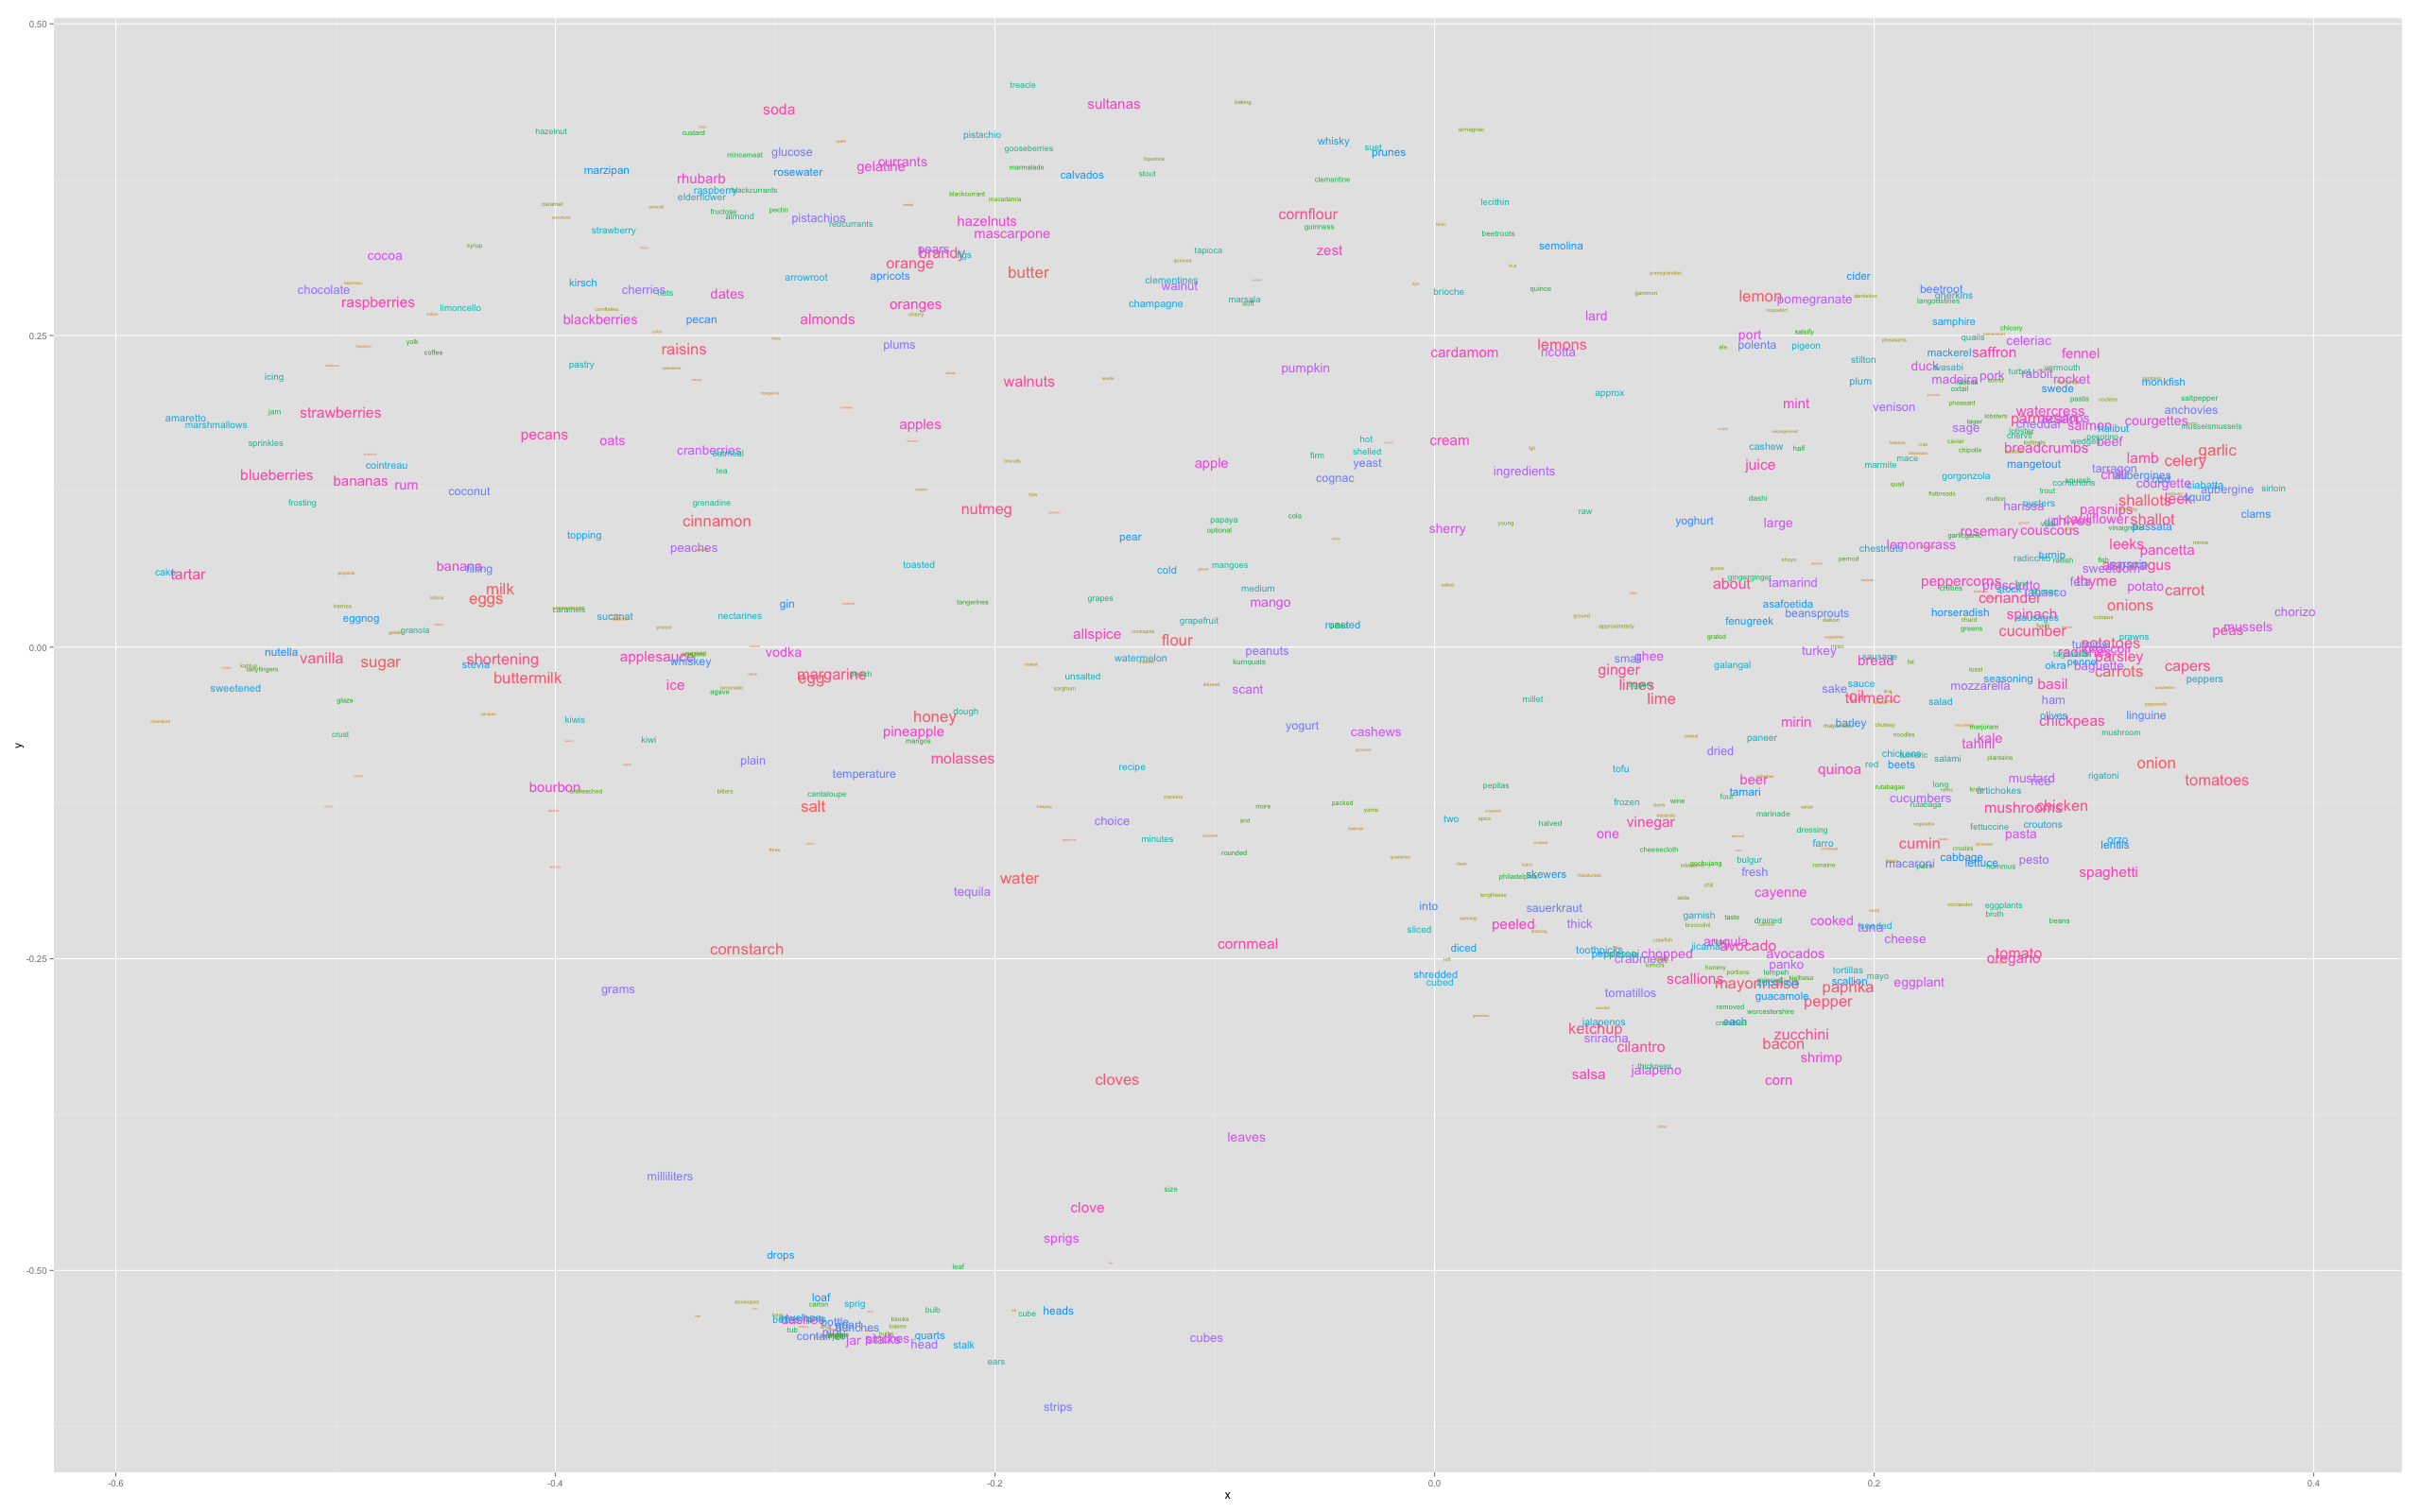
\includegraphics[width=0.95\colwidth]{wallpaper.png}}
        \column{0.5}
        \block{Composition}{
            We can compose a given list of ingredients by summing up the vectors individually. In this way, we constructed a second recipe space (\textbf{ComposedRecipes}). Next, we can find similar recipe vectors to the one constructed by adding ingredient vectors.

        \vspace{3cm}

            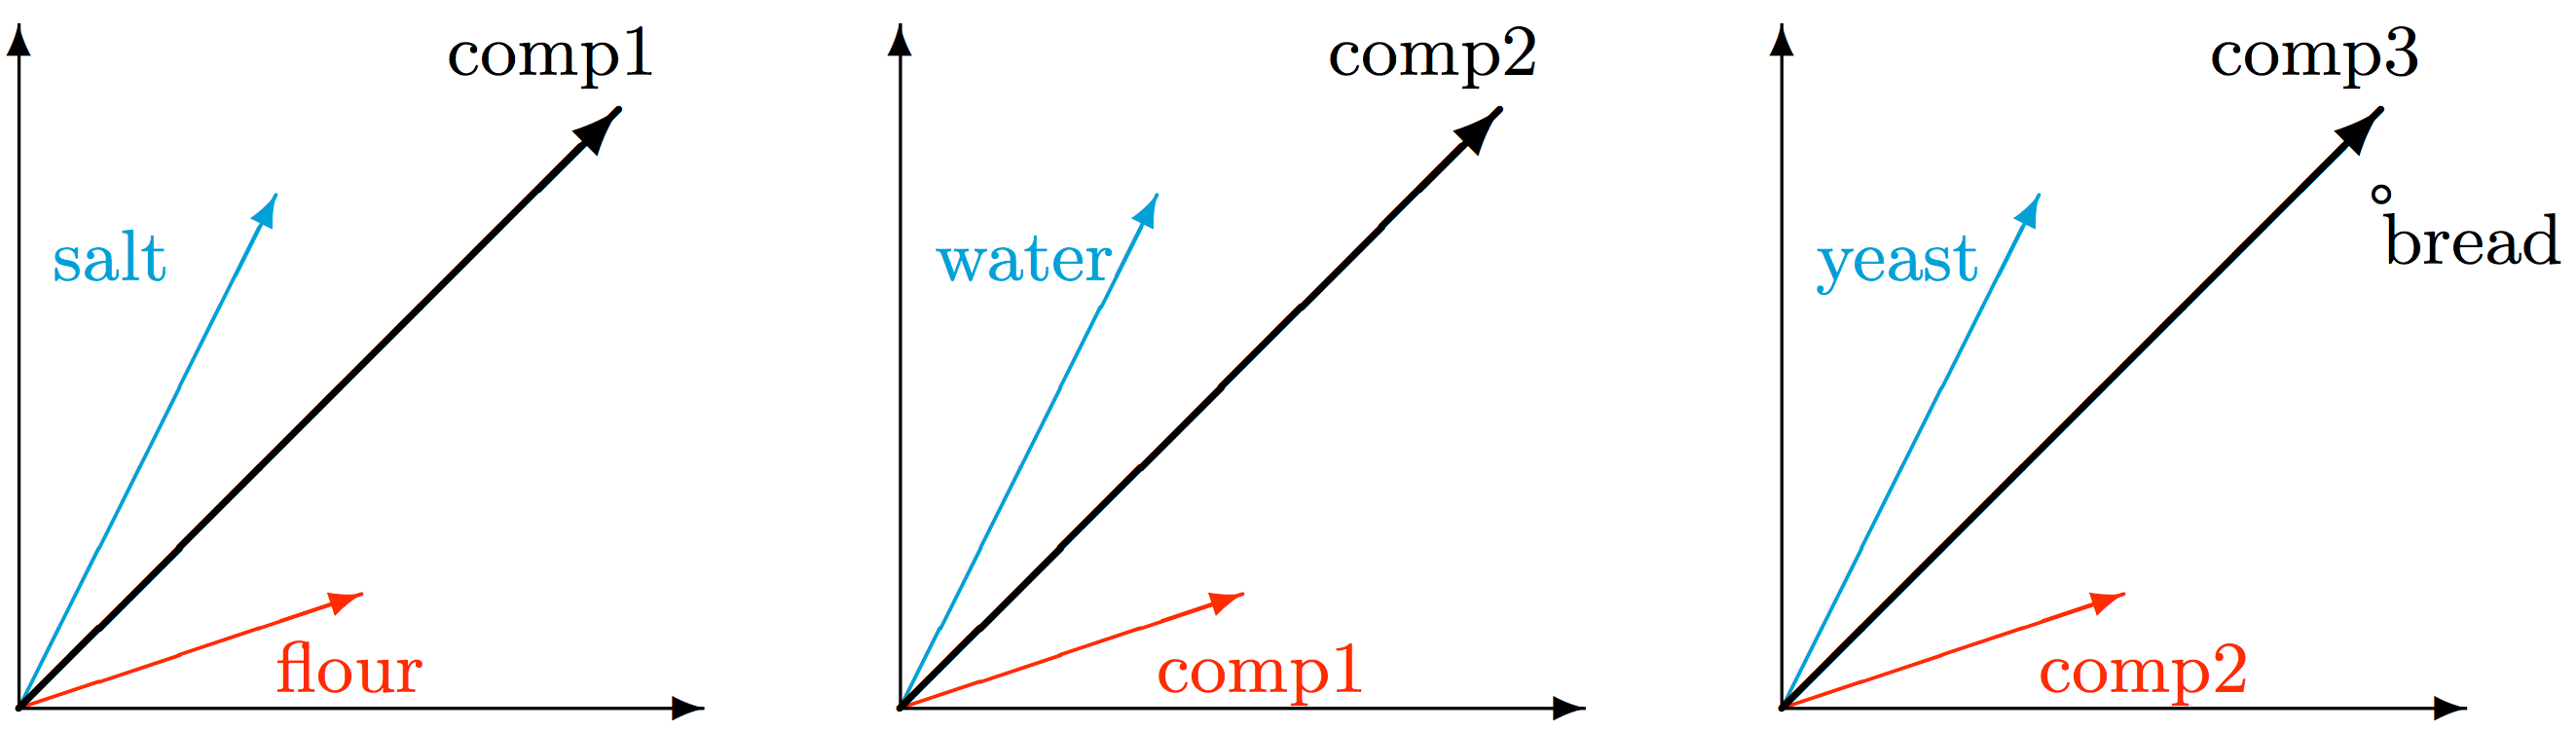
\includegraphics[width=0.95\colwidth]{figure2.png}
            \vspace{1cm}
            \begin{center}
             $\overrightarrow{bread} \approx \overrightarrow{flour} + \overrightarrow{salt} + \overrightarrow{water} + \overrightarrow{yeast}$
            \end{center}
 }
        \block{Results \& Trying Evaluation}{
            Subjectively evaluated, the resulting spaces seem to produce good results, when looking at the nearest neighbors of ingredients. As a similarity measure, we use the \textit{cosine distance}:

            \begin{center}
                \begin{equation*}
                    cos(\overright{u},\overright{v}) = \frac{<\overright{u},\overright{v}>}{\sqrt{||\overright{u}||\,||\overright{v}||}}
                \end{equation*}

            \vspace{1cm}

            \begin{tabular}{cc}
                \toprule
                \textbf{Input ingredient} & \textbf{Nearest neighbors}\\
                \midrule
                flour & warm water, egg yolk, nutmeg\\
                milk & melted butter, butter or margarine, eggs\\
                mozzarella & basil, pasta, freshly grated parmesan\\
                blueberries & frozen mixed berries, peaches, strawberries\\
                \bottomrule
            \end{tabular}
            \end{center}

            \vspace{1cm}

        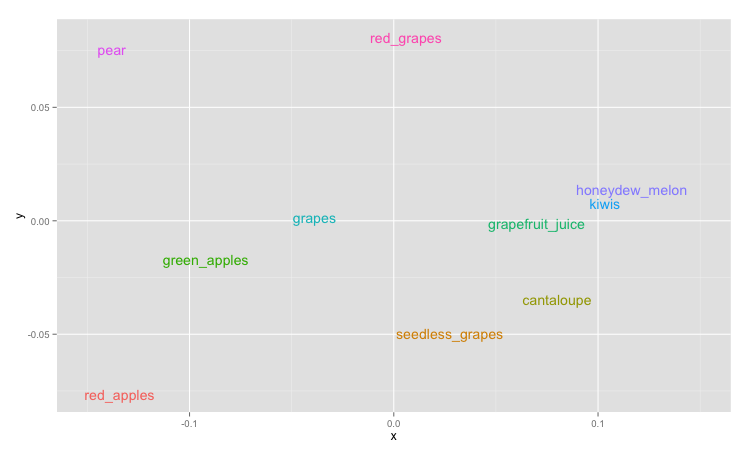
\includegraphics[width=0.475\colwidth]{grapes_final.png}
        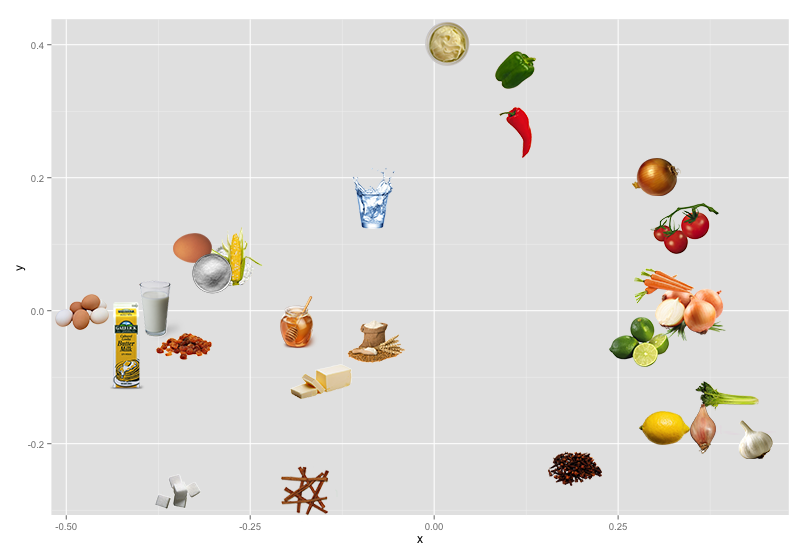
\includegraphics[width=0.475\colwidth]{ingredipic.png}

            Evaluation through \textbf{WordNet} was tried, but no significant link between our similarity and \textit{Path distance} or \textit{JCN distance} could be found. This is not very surprising, since WordNet's hierarchy is unrelated to how ingredients are used in cooking. For example, while \textit{butter} and \textit{margerine} are often used interchangably, they are very different things.
        \vspace{2cm}

        Two scripts were created to experiment with our semantic gastrospaces:
        \vspace{1cm}


            \raisebox{.768\height}{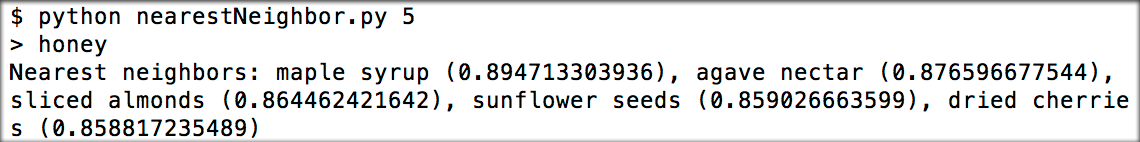
\includegraphics[width=0.475\colwidth]{nn.png}}
            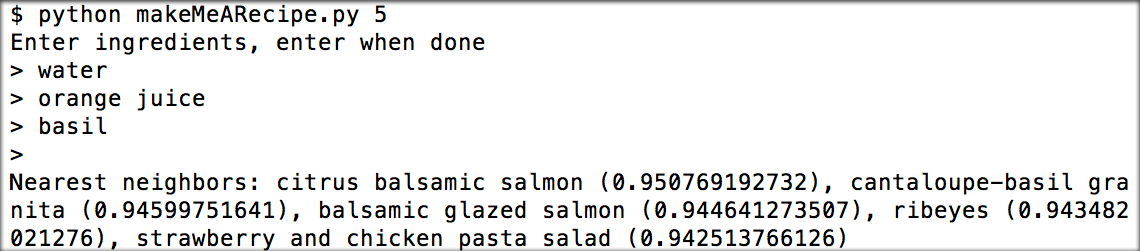
\includegraphics[width=0.475\colwidth]{mmar.png}
        }
        \block{Future Work}{
            %Two scripts have been created for demonstration:
            \begin{itemize}
                \item Additional cleaning \& unification
                \item Composition weighting based on ingredient amounts
                \item Experimenting with other composition methods, e.g. Multiplicative
                \item Finding better methods of automatic evaluation
                \item Make use of additional information in recipe data, e.g. cooking process
                \item Twitter-Bot or App for Make-Me-A-Recipe
            \end{itemize}
            
\includegraphics[width=0.9\colwidth]{esslli.png}
        }
    \end{columns}
\end{document}
